%!TEX root = these.tex

\chapter{Offline Evaluation of LTL Formulæ with Bitmap Manipulations}

This chapter represents a modified version of a paper which is written by K. Xie and S. Hallé and still under review for publication in the proceedings of the International Conference: Runtime Verification 2016 (RV'16) in Madrid, Spain in 2016.

%% ------------------
%% Section: intro
%% ------------------
\section{Introduction}\label{sec:bm:intro} %% {{{

\emph{Temporal logic} \cite{huth2004} is a logistic system which uses rules and symbols to describe and reason about the change of a system's state in terms of time. It is based on the idea that one state may not be constantly true or false as time goes. \emph{Linear Temporal Logic (LTL)} \citep{pnueli97} is a temporal logic, and as its name entails, \emph{LTL} can denote only one sequence of states and for each state there is only one future state.

A \emph{bitmap}, also known as a bit array or bitset, is a compact data structure storing a sequence of binary values. As will be shown in Section \ref{sec:bm:compression}, it can be used to express a set of numbers, or an array where each bit represents a 2-valued option. Bitmaps present several advantages as a data structure: they can concisely represent information, and provide very efficient functions to manipulate them, taking advantage of the fact that multiple bits can be processed in parallel in a single CPU instruction.

In this paper, we explore the idea of using bitmap manipulations for the offline evaluation of LTL formul\ae{} on an event log. For this purpose, in Section \ref{sec:bm:ltlbitmap}, we introduce a solution which, for a given event trace $\sigma$ and an LTL formula $\varphi$, first converts each ground term into as many bitmaps; intuitively, the bitmap for atomic proposition $p$ describes which events of $\sigma$ satisfy $p$. Algorithms are then detailed for each LTL operator, taking bitmaps as their input and returning a bitmap as their output. The recursive application of these algorithms can be used to evaluate any LTL formula.

This solution presents several advantages. First, the use of bitmaps can be seen as a form of \emph{indexing} (in the database sense of the term) of a trace's content. Rather than being an online algorithm merely reading a pre-recorded trace, our solution exploits the fact that the trace is completely known in advance, and makes extensive use of this index to jump to specific locations in the trace to speed up its process. Second, a bitmap having consecutive 0s or 1s can be compressed, which reduces the space cost and speeds up the execution of many operations even further \citep{lemire2014}.

To this end, Section \ref{sec:bm:experiments} describes an experimental setup used to test our solution. It reveals that, that, for complex LTL formul\ae{} containing almost 20 operators, large event traces can be evaluated at a throughput of tens of millions of events per second.

%% }}} --- Section

%% ------------------
%% Section: bitmap compression
%% ------------------
\section{Bitmaps and Compression}\label{sec:bm:compression} %% {{{

A bitmap (or bitset) is a binary array that we can view as an efficient and compact representation of an integer set. Given a bitmap of $n$ bits, the $i$-th bit is set to 1 if the $i$-th integer in the range $[0, n-1]$ exists in the set. The union and intersection between these sets can be computed using bitwise operations (OR, AND) on the bitmaps.

A bitmap can map from $n$ chunks of data into $n$ bits. If the size of each chunk is greater than 1, the bitmap can greatly reduce the size of the storage. And With its power of exploiting bit-level parallelism in hardware, its operations can be very efficient. Therefore bitmap has a lot of applications of which the requirement of space or efficiency is essential, for example, information retrieval \citep{Chan:1998:BID:276305.276336}, database \citep{burdick2001mafia}, and data mining \citep{Ayres:2002:SPM:775047.775109} \citep{Uno:2005:LVC:1133905.1133916}.

A bitmap with low fraction of 1 bits can be considered sparse \citep{lemire2014}. A sparse bitmap without compression is a waste in both time and space. There are many popular compression algorithms are based on the Run-Length Encoding (RLE) model derived from BBC\citep{antoshenkov1995byte}. We briefly describe a few of these techniques in the following.  We choose WAH\citep{wu2006optimizing}, Concise\citep{colantonio2010} and EWAH\citep{lemire2010} because they have well-implemented Open Source libraries in Java.

\subsection{WAH}

WAH \citep{wu2006optimizing} divides a bitmap of $n$ bits into $\lceil \frac{n}{w-1}\rceil$ words of $w -1$ bits, where $w$ is a convenient word length (for example, 32). WAH distinguishes between two types of words: words made of just
$w-1$ ones ($11\dots 1$) or just $w-1$ zeros ($00\dots 0$), are \emph{fill words}, whereas words containing a mix of zeros and ones are \emph{literal words}. Literal words are stored using $w$ bits: the most significant bit is set to zero and the remaining bits store the heterogeneous $w-1$ bits. Sequences of homogeneous fill words (all ones or all zeros) are also stored using w bits: the most significant bit is set to 1, the second most significant bit indicates the bit value of the homogeneous block sequence, while the remaining $w-2$ bits store the run length of the homogeneous block sequence.

\subsection{Concise}

Concise \citep{colantonio2010} is a bitmap compression algorithm based on WAH. Comparing with WAH of which the run length is $w-2$ bits, Concise uses $w - 2 - \lceil \log_2 w \rceil$ for the run length and $\lceil \log_2 w \rceil$ bits to store an integer value indicating to flip a bit of a single word of $w-1$ bits. This feature can improve the compression ratio in the worst case.

\subsection{EWAH}

EWAH \citep{lemire2010} is also a variant of WAH but it does not use its first bit to indicate the type of the word like WAH and Concise. EWAH defines a $w$-bits marker word. The most significant $w/2$ bits of the word are used to store the number of the following fill words (all ones or all zeros) and the rest $w/2$ bits entails the number of the dirty words which are exactly like the literal words of WAH but the dirty words of EWAH utilize all $w$ bits. With this structure, a single word in the sequences is difficult to be recognized as a marker word or a dirty word unless the word is the first one, and thus a reverse enumeration is nearly impossible.

\subsection{Roaring}

Besides the RLE-model algorithms, there are other bitmap compression model which supports fast random access like the uncompressed bitmap does. One of them is Roaring bitmap.

Roaring bitmap \citep{lemire2015} has a compact and efficient two-level indexing data structure which splits 32-bit indexes into chunks, each of which stores the 16 most significant bits of a 32-bit integer and points to a specialized container storing the 16 least significant bits. There are two types of containers: a sorted 16-bit integer array for \emph{sparse} chunks which store at maximum 4096 integers, and a bitmap for \emph{dense} chunks which store $(4096, 2^{16})$ integers. This hybrid data structure allows to fast random access whereas all RLE-model algorithms mentioned cannot because of their own characteristics.

%The time complexities of the LTL operators with \emph{Roaring bitmap} are $O(n)$ because we cannot skip certain bits when enumerating the bitmap.

\subsection{Discussion}

The RLE-model algorithms share some common features and also have their own characteristics. First, all of them have two different kinds of words, one of which is to store the raw uncompressed word (literal word) and the other is compressed word (sequence word) having a bit and a number. The number represents the number of consecutive words which are full of 0s or 1s determined by the bit.

We use $wlen$ to represent the number of bits in a word, $ulen$ the number of available in a literal word and $wcap$ the maximum number of bits stored in a sequence word. Table \ref{tbl:bm:bmparms} lists the parameters of the three RLE-model algorithms.

\begin{table}[h]
\centering
\begin{tabular}{|c|c|c|c|}
\hline
& ulen & wlen & wcap \\
\hline
WAH & 31 bits & 32 bits & $2^{30} - 1$ \\
\hline
Concise & 31 bits & 32 bits & $2^{25} - 1$ \\
\hline
EWAH & 32 or 64 bits & 32 or 64 bits & $2^{16} - 1 \text{ or } 2^{32} - 1$ \\
\hline
\end{tabular}
\caption{Parameters of RLE-model algorithms}
\label{tbl:bm:bmparms}
\end{table}

Considering that a $n$-bits bitmap has $m$ sequences of consecutive (0...1...) bits:
\begin{align*}
& c^1_0c^0_1c^1_1c^0_1c^1_2c^0_2...c^1_{m - 1}c^0_{m - 1}, c^i_j \text{ is the number of } \\
& \text{consecutive } i \text{ bits and } i \in (0, 1),\, 0 \leq j \leq m.  
\end{align*}

Then the number of total bits, i.e. the size of the uncompressed bitmap is:
\begin{align*}
& total\_bits = \sum_{j = 0}^{m - 1} \sum_{i = 0}^1 c^i_j = \sum_{j = 0}^{m - 1} \sum_{i = 0}^1 l^i_j + s^i_j, \\
& l^i_j = c^i_j \text{ mod } ulen, s^i_j = c^i_j - l^i_j
\end{align*}

If exists a positive integer $slen$, $\forall c^i_j = slen$, then
\begin{align}
m = n \div (2 \times slen) \label{eq:seqnum}
\end{align}

When $1 \leq slen < wlen$, then $\forall l^i_j > 0, \forall s^i_j = 0$, which is considered the worst case, the size of the compressed bitmap is:
\begin{align*}
compressed\_bits = \lceil \frac{total\_bits}{ulen} \rceil \times wlen 
\end{align*}

None of the three RLE-model algorithms can well compress this kind of bitmap. Both \emph{WAH} and \emph{Concise} waste one bit for the type identification and \emph{EWAH} seems to cost the least for its $ulen = wlen$ but its actual size should be a little more than $total\_bits$ because some empty sequence word is needed to store the number of the literal words.

Furthermore, when $wlen \leq slen$, then $\forall s^i_j > 0$, the sequence can be well compressed with any RLE-model algorithm. Suppose $\forall l^i_j > 0$, the size of the compressed bitmap is:
\begin{align*}
compressed\_bits = &\sum_{j = 0}^{m - 1} \sum_{i = 0}^1 \lceil \frac{slen}{wcap} \rceil \times wlen + wlen \\
= & 2 \times m \times wlen \times (1 + \lceil \frac{slen}{wcap} \rceil)
\end{align*}

From this discussion, we can see that $slen$, i.e. the number of consecutive 1 or 0 bits in a sequence, is a crucial argument and is able to decide the compression rate of a RLE bitmap compression algorithm. Some optimization like Concise is merely to try to improve the performance of the worst case.

%% }}} --- Section

%% ------------------
%% Section: algos
%% ------------------
\section{Calculate LTL formul\ae{} with Bitmap}\label{sec:bm:ltlbitmap} %% {{{

In this section we introduce our solution of mapping LTL states to bitmaps and calculating the formul\ae{} with the mapped bitmaps.

\subsection{Manipulate bitmaps to implement LTL operators} %% {{{

Given a finite $n$-states sequence of states $(s_0, s_1, ..., s_{n - 1})$ and an LTL formula $L$, a $n$-bits bitmap defined as Definition \eqref{eq:map} is dedicated to store the bits which indicate whether the corresponding paths satisfy the formula. The bitmap mapping from the formula $L$ is called $B_l$.

\begin{equation}\label{eq:map}
(b_0b_1...b_ib_{i + 1}...b_{n - 1})_n, b_i = \begin{cases}
1, & \text{if $\pi^i \vDash L$} \\
0, & \text{otherwise}
\end{cases}
\end{equation}

We suppose that a well-designed data structure of bitmap has certain basic functions. Given bitmaps $a$, $b$, we will note $|a|$ the function that computes the length of $a$. The notation $a \otimes b$ will denote the bitwise logical AND of $a$ and $b$, $a \oplus b$ the bitwise logical OR, and $!a$ its bitwise inverse. % as are described in Table \ref{tbl:bm:bmfuncs}.

% \begin{table}
% \centering
% \begin{tabular}{|l|l|}
% \hline
% Function & Description \\
% \hline
% $|b|$ & gets the size of the bitmap. \\
% % \hline
% % get(bitmap, index) & gets the true/false value from the specific index in the bitmap. % PAS UTILISÉE DANS LES ALGOS \\
% % \hline
% % set(bitmap, index, val) & sets the true/false value to the specific index in the bitmap. % PAS UTILISÉE NON PLUS \\
% % \hline
% % and(bitmap1, bitmap2) & performs a logic $\mathit{AND}(\wedge)$ operation of the two input bitmaps. \\
% \hline
% or(bitmap1, bitmap2) & performs a logic $\mathit{OR}(\vee)$ operation of the two input bitmaps. \\
% \hline
% not(bitmap) & performs a logic $\mathit{NOT}(\neg)$ operation of the input bitmap. \\
% \hline
% \end{tabular}
% \caption{Basic bitmap functions}
% \label{tbl:bm:bmfuncs}
% \end{table}

These bitmap functions are enough to implement the LTL operators, but in order to optimize our solution and integrate with bitmap compression algorithms shown in Section \ref{sec:bm:compression}, we need to manipulate the internal data structure of the bitmap and thus introduce 7 derivative bitmap functions (See Table \ref{tbl:bm:bmhelpers}).
\begin{table}
\centering
\begin{tabular}{|l|p{8cm}|}
\hline
Function & Description \\
\hline
addMany(bitmap, val, len) & adds a $len$-bits sequence of the same value to the end of the bitmap whose size then increases by $len$. \\
\hline
copyTo(bitmapDest, bitmapSrc, start, len) & copies the $len$-bits sequence from the index $start$ in bitmap $bitmapSrc$ to the end of another bitmap $bitmapDest$ whose size then increases by $len$. \\
\hline
removeFirstBit(bitmap) & removes the first bit of the bitmap, and the size of the bitmap decreases by 1. \\
\hline
next(b, bitmap, start) & gets the position of the next occurrence of the bit with value b from the inclusive position $start$ of the bitmap, or -1 if there is no more. \\
% \hline
% next(1, bitmap, start) & gets the position of the next occurrence of the bit "1" from the inclusive position $start$ of the bitmap, or -1 if there is no more "1". \\
\hline
last(b, bitmap) & gets the position of last occurrence of the bit with value b in the bitmap, or -1 if the bitmap does not have a bit with value b. \\
% \hline
% last(1, bitmap) & gets the position of last occurrence of the bit "1" in the bitmap, or -1 if the bitmap does not have a bit "1". \\
\hline
\end{tabular}
\caption{Derivative bitmap functions}
\label{tbl:bm:bmhelpers}
\end{table}

The finite set of atomic propositions constitute the initial bitmaps. Consider a $n$-states sequence, according to Definition \eqref{eq:ap}, the bit $b_i$ of $B_p$ is set to $1$ if the atomic proposition is true at the corresponding state $s_i$, otherwise 0.

Conjunction, disjunction and negation have their direct equivalents as bitwise operators, and the remaining propositional connectives can be easily reduced to these three through standard identities. % Propositional logic operators have their direct translated to bitwise operators. The functions $\mathop{not}(), \mathop{and}(), \mathop{or}()$ from the bitmap are enough to the calculation of the formul\ae{} $\neg\psi$\eqref{eq:not}, $\psi \wedge \varphi$\eqref{eq:and}, $\psi \vee \varphi$\eqref{eq:or}. And the formula $\psi \rightarrow \varphi$ can be expanded to $\neg \psi \vee \varphi$ \cite{huth2004}.
% 
% \begin{align*}
% \neg \psi &\mapsto \mathop{not}(B_\psi) \\
% \psi \wedge \varphi &\mapsto \mathop{and}(B_\psi, B_\varphi) \\
% \psi \vee \varphi &\mapsto \mathop{or}(B_\psi, B_\varphi) \\
% \psi \rightarrow \varphi &\mapsto \mathop{or}(\mathop{not}(B_\psi), B_\varphi) \\
% \end{align*}
%
Temporal logic operators are a little more complicated because they concern the change of the states in terms of time, therefore we have to enumerate the actual states and the bits in the bitmaps.

Definition \eqref{eq:next} states that the operator $\mathop{X}$ aims to check if the next state of a state is fine, so for a sequence of states, we just need to remove the first state and the rest states immediately become the "next" states. For the corresponding bitmap, we remove its first bit (see Algorithm \ref{alg:next}).

\begin{figure}
\centering
\subfloat[$\mbox{\bf X}\,\varphi$]{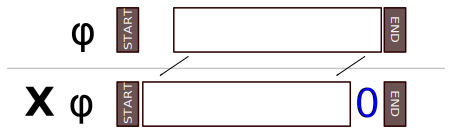
\includegraphics[scale=0.3]{Pattern-X}}~~~
\subfloat[$\mbox{\bf G}\,\varphi$]{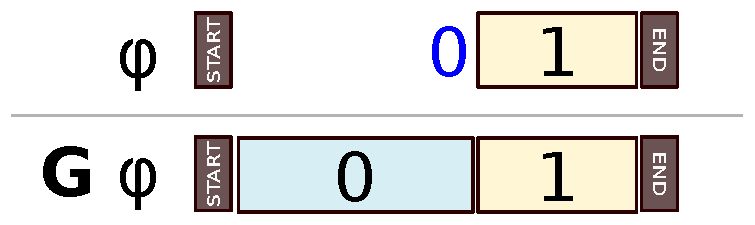
\includegraphics[scale=0.3]{Pattern-G}}~~~
\subfloat[$\varphi\,\mbox{\bf U}\,\psi$]{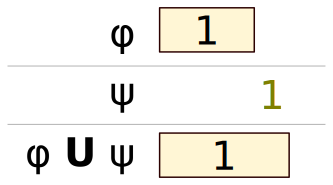
\includegraphics[scale=0.3]{Pattern-U}}
\caption{A graphical representation of the computation of three temporal operators on bitmaps}
\label{fig:patterns}
\end{figure}

\begin{algorithm}
\caption{Computing $\X a$}
\label{alg:next}
\begin{algorithmic}[1]
\Require Bitmap $a$
%\State // X(10101) $\Rightarrow$ (0101)
\State $out \gets$ removeFirstBit($a$)
\State addMany($out$, 0, 1)
\State \Return $out$
\end{algorithmic}
\end{algorithm}

The dual formul\ae{} $\mathop{G}\psi$ and $\mathop{F}\psi$ demand to find the $i$-th path $\pi^i$ from which on all the following paths $\pi^{i + 1}, \pi^{i + 2}, ... \pi^n$ relatively satisfy or do not satisfy the formula $\psi$, according to Definition \eqref{eq:global} and \eqref{eq:future}. Thus to implement these two formul\ae{} with bitmap, we need to do a search in the bitmap $B_{\psi}$ from back to front to find the last occurrence of the bit "0" or "1", as can be seen from Algorithm \ref{alg:global} and Algorithm \ref{alg:future}.

\begin{algorithm}
\caption{Computing $\G a$}
\label{alg:global}
\begin{algorithmic}[1]
\Require Bitmap $a$
\State $p \gets$ last(0, $a$)
\If {$p = -1$}
  \State \Return $a$
\Else
  \State $out \gets \langle~\rangle$
  \State addMany($out$, 0, $p + 1$)
  \State addMany($out$, 1, $|a| - p - 1$)
  \State \Return $out$
\EndIf
\end{algorithmic}
\end{algorithm}

\begin{algorithm}
\caption{\textbf{F}uture}
\label{alg:future}
\begin{algorithmic}[1]
\Require Bitmap $a$
%\State // F(010100) $\Rightarrow$ (111100)
\State $pos \gets$ last(1, $a$)
\If {$pos = -1$}
  \State \Return $a$
\Else
  \State $out \gets$ empty Bitmap
  \State addMany($out$, 1, $pos + 1$)
  \State addMany($out$, 0, $|a| - pos - 1$)
  \State \Return $out$
\EndIf
\end{algorithmic}
\end{algorithm}

According to Definition \eqref{eq:until}, if there is a $\pi^j$ which satisfies $\varphi$ and the paths $\pi^i, \pi^{i + 1}, ... \pi^{j - 1}$ all satisfy $\psi$, the path $\pi^i$ must satisfy the formula $\psi \mathrel{U} \varphi$. With respect to the operation of bitmaps, we need to keep checking if there is any bit set as 1 in $B_{\psi}$ before the every occurrence of bit 1 in $B_{\varphi}$ (see Algorithm \ref{alg:until}).

\begin{algorithm}
\caption{Computing $a \U b$}
\label{alg:until}
\begin{multicols}{2}
\begin{algorithmic}[1]
\Require Bitmaps $a$ and $b$
\State $out \gets \langle~\rangle$
\State $p, a_0, a_1, b_0, b_1 \gets 0$
\While {$p < |a|$}
  \If {$a_1 \leq p$}
    \State $a_1 \gets$ next(1, $a$, $p$)
  \EndIf

  \If {$b_1 \leq p$}
    \State $b_1 \gets$ next(1, $b$, $p$)
  \EndIf

  \If {$a_1 = -1$ or $b_1 = -1$}
    \State \textbf{break}
  \EndIf

  \State $nearest1 \gets$ min($a_1$, $b_1$)
  \If {$nearest1 > p$}
    %\State // (00..) U (00..) $\Rightarrow$ (00..)
    \State addMany($out$, 0, $nearest1 - p$)
    \State $p \gets nearest1$
    \State \textbf{continue}
  \EndIf

  \If {$p = b_1$}
    %\State // (??..) U (11..) $\Rightarrow$ (11..)
    \If {$b_0 \leq b_1$}
      \State $b_0 \gets$ next(0, $b$, $b_1$)
      \If {$b_0 = -1$}
        \State $b_0 \gets |a|$
      \EndIf
    \EndIf
    \State addMany($out$, 1, $b_0 - p$)
    \State $p \gets b_0$
    \State \textbf{continue}
  \EndIf

  \If {$a_0 \leq a_1$}
    \State $a_0 \gets$ next(0, $a$, $a_1$)
    \If {$a_0 = -1$}
      \State $a_0 \gets |a|$
    \EndIf
  \EndIf
  \If {$a_0 \geq b_1$}
    %\State // (111?..) U (0001..) $\Rightarrow$ (1111..)
    \State addMany($out$, 1, $b_1 - p + 1$)
    \State $p \gets b_1 + 1$
  \Else
    %\State // (11100..) U (00001..) $\Rightarrow$ (00000..)
    \State addMany($out$, 0, $a_0 - p + 1$)
    \State $p \gets a_0 + 1$
  \EndIf
\EndWhile

\If {$b_1 = -1$}
  %\State // (..??) U (..00) $\Rightarrow$ (..00)
  \State addMany($out$, 0, $|a| - |out|$))
\ElsIf {$a_1 = -1$}
  %\State // (..0000) U (..1010) $\Rightarrow$ (..1010)
  \State copyTo($out$, $b$, $p$, $|a| - p$)
\EndIf

\State \Return $out$
\end{algorithmic}
  \end{multicols}
\end{algorithm}

The operation $\psi \textbf{ W } \varphi$ (Definition \eqref{eq:wuntil}) is quite like $\psi \textbf{ U } \varphi$, except that as the equation \eqref{eq:uw} \citep{huth2004} entails, the operation of the former also includes the operation $\textbf{G}\psi$. Algorithm \ref{alg:wuntil} explains its operation.

\begin{equation} \label{eq:uw}
\psi \textbf{W} \varphi \equiv \psi \textbf{U} \varphi \vee \textbf{G}\psi
\end{equation}

\begin{algorithm}
\caption{Computing $a \W b$}
\label{alg:wuntil}
\begin{multicols}{2}
\begin{algorithmic}[1]
\Require Bitmaps $a$ and $b$
\State $out \gets \langle~\rangle$
\State $p, a_0, a_1, b_0, b_1 \gets 0$
\While {p < |a|}
  \If {$a_1 \leq p$}
    \State $a_1 \gets$ next(1, $a$, $p$)
  \EndIf
  \If {$b_1 \leq p$}
    \State $b_1 \gets$ next(1, $b$, $p$)
  \EndIf
  \If {$a_1 = -1$ or $b_1 = -1$}
    \State \textbf{break}
  \EndIf

  \State $nearest1 \gets$ min($a_1$, $b_1$)
  \If {$nearest1 > p$}
    \State addMany($out$, 0, $nearest1 - p$)
    \State $p \gets nearest1$
    \State \textbf{continue}
  \EndIf

  \If {$p = b_1$}
    \If {$b_0 \leq b_1$}
      \State $b_0 \gets$ next(0, $b$, $b_1$)
      \If {$b_0 = -1$}
        \State $b_0 \gets |a|$
      \EndIf
    \EndIf
    \State addMany($out$, 1, $b_0 - p$)
    \State $p \gets b_0$
    \State \textbf{continue}
  \EndIf

  \If {$a_0 \leq a_1$}
    \State  $a_0 \gets$ next(0, $a$, $a_1$)
    \If {$a_0 = -1$}
      \State $a_0 \gets |a|$
    \EndIf
  \EndIf

  \If {$a_0 \geq b_1$}
    \State addMany($out$, 1, $b_1 - p + 1$)
    \State $p \gets b_1 + 1$
  \Else
    \State addMany($out$, 0, $a_0 - p + 1$)
    \State $p \gets a_0 + 1$
  \EndIf
\EndWhile

\If {$b_1 = -1$}
  \If {$a_1 = -1$}
    \State addMany($out$, 0, $|a| - |out|$)
  \Else
    \State $last0 \gets$ last(0, $a$)
    \If {$last0 = -1$ or $last0 < p$}
      \State addMany($out$, 1, $|a| - |out|$)
    \Else
      \State addMany($out$, 0, $last0 - p + 1$)
      \State addMany($out$, 1, $|a| - |out|$)
    \EndIf
  \EndIf
\ElsIf {$a_1 = -1$}
  \State copyTo($out$, $b$, $|b| - b_1 - 1$, $|b| - b_1$)
\EndIf

\State \Return $out$
\end{algorithmic}
\end{multicols}
\end{algorithm}

As the dual of the operator \textbf{U}, the operator \textbf{R} defined in \eqref{eq:release} need to union two parts for the formula $\psi \textbf{R} \varphi$: the first part aims to find whether exist $i, j (0 \leq i < j)$ which make $\pi^i, \pi^{i + 1}, ... \pi^j$ satisfy $\varphi$ when $\pi^j$ satisfies $\psi$; and the second is simply $G\varphi$. Algorithm \ref{alg:release} describes this procedure.

\begin{algorithm}
\caption{Computing $a \R b$}
\label{alg:release}
\begin{multicols}{2}
\begin{algorithmic}[1]
\Require Bitmaps $a$ and $b$
\State $out \gets \langle~\rangle$
\State $p, a_0, a_1, b_0, b_1 \gets 0$
\While {$p < |a|$}
  \If {$b_1 \leq p$}
    \State $b_1 \gets$ next(1, $b$, $p$)
  \EndIf
  \If {$b_1 = -1$}
    \State \textbf{break}
  \EndIf

  \If {$b_1 > p$}
    \State addMany($out$, 0, $b_1 - p$)
    \State $p \gets b_1$
    \State \textbf{continue}
  \EndIf

  \If {$a_1 \leq p$}
    \State $a_1 \gets$ next(1, $a$, $p$)
  \EndIf
  \If {$a_1 = -1$}
    \State \textbf{break}
  \EndIf

  \If {$b_0 \leq b_1$}
    \State $b_0 \gets$ next(0, $b$, $b_1$)
    \If {$b_0 = -1$}
      \State $b_0 \gets |a|$
    \EndIf
  \EndIf
  \If {$a_1 \geq b_0$}
    \State addMany($out$, 0, $b_0 - p + 1$)
    \State $p \gets b_0 + 1$
    \State \textbf{continue}
  \EndIf

  \If {$a_0 \leq a_1$}
    \State $a_0 \gets$ next(0, $b$, $a_1$)
    \If {$a_0 = -1$}
      \State $a_0 \gets |a|$
    \EndIf
  \EndIf
  \State $nearest0 \gets$ min($a_0$, $b_0$)
  \State addMany($out$, 1, $nearest0 - p$)
  \State $p \gets nearest0$
\EndWhile

\If {$a_1 = -1$ and $b_1 \neq -1$}
  \State $last0 \gets$ last(0, $b$)
  \If {$last0 = -1$ and $last0 < p$}
    \State addMany($out$, 1, $|a| - |out|$)
  \Else
    \State addMany($out$, 0, $last0 - p + 1$)
    \State addMany($out$, 1, $|a| - |out$)
  \EndIf
\Else
  \State addMany($out$, 0, $|a| - |out|$)
\EndIf

\State \Return $out$
\end{algorithmic}
\end{multicols}
\end{algorithm}

\subsection{Discussion}

An interesting point of this last algorithm is that the bitmaps $a$ and $b$ are not traversed in a linear fashion. Rather, entire blocks of each bitmap can be skipped to reach directly the next 0 or the next 1, depending on the case. Note that this is only possible if the trace is completely known in advance before starting to evaluate a formula. Therefore, our proposed solution is an example of an offline monitor that is not simply an online monitor that is fed events of a pre-recorded trace one by one: it exploits the possibility of \emph{random access} to parts of the trace which is only possible in an offline setting.

As is indicated in this section, the time complexities of all operators including propositional logic operators and temporal operators are $O(n)$ and the space complexities are also $O(n)$ where $n$ is the size of the input bitmap.

For the bitmap mapping from the states, certain operators lean to generate the result bitmap which has longer runs of consecutive 0s or 1s than the input ones. The operators \textbf{F} and \textbf{G} output the bitmap which has at most two sequences of consecutive 0s or 1s. The operators \textbf{U}, \textbf{W} and \textbf{R} have the ability to combine the continuous 1s from the two input bitmaps to get a longer sequence of 1s. Thus we introduced bitmap compression in our solution to see if there is any improvement.

%% }}} --- Subsection

%% }}} --- Section

%% ------------------
%% Section: expériences
%% ------------------
\section{Implementation and Experiments}\label{sec:bm:experiments} %% {{{

In this section, we describe experiments in order to achieve the following purposes:
\begin{enumerate}
\item Test the performance of fundamental LTL operators;
\item Test the performance of complicated LTL formul\ae{};
\item Test the performance of LTL formula with compressed bitmaps;
\item Observe the compression ratio of bitmap compression algorithms.
\end{enumerate}

\subsection{Modifications to Libraries} %% {{{

Section \ref{sec:bm:ltlbitmap} mentions that the time and space complexities of all LTL operators are $O(n)$ where $n$ is the size of the input uncompressed bitmap. After applying RLE-model bitmap compression algorithms to our solution, the space complexities become $O(m)$ as is discussed above, and we managed to make the time complexities also become $O(m)$ by implementing the bitmap manipulation functions listed in Table \ref{tbl:bm:bmhelpers} for every  bitmap compression algorithms.

Because of lack of the support of random access for the RLE-model bitmap compression algorithms, we cannot enumerate the bits in the same way as uncompressed bitmap. Therefore we design an \emph{iterator} data structure to store not only the absolute index of current bit in the uncompressed bitmap but also the relative index in the compressed bitmap.

Taking the function \textbf{next(1, )} as an example, if the current relative index is in a sequence word of 0, the search in this word is unnecessary, and we just jump to the next word; if the index is in a sequence word of 1, we return the current index; however, if the index is in a literal word, we have to look for the bit 1 in the $ulen$-bits word.

%% }}}

\subsection{Experimental Setup} %% {{{

As a means to avoid the runtime disk I/O cost we load all relevant files into memory before the calculations. Thus although using bitmap can considerably reduce the requirement of memory, we prepared a workstation with an Intel Xeon E5-2630 v3 Processor and 48 GB of memory.

All codes are implemented in Java which self takes responsibility of the memory management and garbage collection. Concerning the delay caused by garbage collection (GC) and especially Full-GC, we called \textit{System.gc()} before and after every formula calculation to provide a runtime environment that was as ``clean'' as possible.

Table \ref{table:bmlibs} shows the libraries used for different types of bitmap. In order to implement all the LTL operations, we modified the codes of the libraries to add the necessary functions listed in Table \ref{tbl:bm:bmhelpers} and to optimize the functions so that the time complexities of the operators become $O(m)$ where $m$ is the number of sequences of consecutive 0/1 bits.

\begin{table}
\centering
\begin{tabular}{|c|l|}
\hline
Bitmap & Source \\
\hline
Uncompressed & \texttt{java.util.BitSet} from Java SDK \\
\hline
\multirow{2}{*}{WAH} & Original:\ \ \url{https://github.com/metamx/extendedset} \\
& Modified: \url{https://github.com/phoenixxie/extendedset} \\
\hline
\multirow{2}{*}{Concise} & Original:\ \ \url{https://github.com/metamx/extendedset} \\
& Modified: \url{https://github.com/phoenixxie/extendedset} \\
\hline
\multirow{2}{*}{EWAH} & Original:\ \ \url{https://github.com/lemire/javaewah} \\
& Modified: \url{https://github.com/phoenixxie/javaewah} \\
\hline
Roaring & \url{https://github.com/lemire/RoaringBitmap} \\
\hline
\end{tabular}
\caption{Bitmap libraries}
\label{table:bmlibs}
\end{table}

For the experiments, we developed a random data generator. Every time it generates $5 \times 10^7$ tuples, and each tuple contains 3 random numbers ($a, b, c$) related with 3 simple inequalities: $a > 0$, $b > 0$ and $c \leq 0$, which will be labelled as $s_0$, $s_1$ and $s_2$, respectively. According to \eqref{eq:ap}, the true/false values of these 3 statements consist of the atomic propositions. When a tuple was passed to the 3 statements, we got 3 boolean values each of which was then turned into a 1/0 bit in the bitmap corresponding to one of the 3 statements. When all tuples were processed, we had 3 bitmaps having 50 million bits each.

The experiment data was a file with 50 million lines of states, each of which contained 3 random numbers used for 3 relational statements. The true/false values of these 3 statements $(s_0, s_1, s_2)$ consisted of the atomic propositions.

% \begin{table}
% \centering
% \begin{tabular}{|c|c|}
% \hline
% & Relational statement \\
% \hline
% $s_0$ & $a > 0$ \\
% \hline
% $s_1$ & $b > 0$ \\
% \hline
% $s_2$ & $c \leq 0$ \\
% \hline
% \end{tabular}
% \caption{Relational statements}
% \label{tbl:bm:statements}
% \end{table}

% Pas vraiment pertinent --SH
% The range of the random numbers is [-10000, 10000], and according to the three inequalities mentioned earlier, it is easy to know that the difference between the probabilities of getting 1 and getting 0 is only about $0.05\permil$ if the random function is fair enough, therefore there should be nearly the same number of 1 and 0 bits in the generated bitmap.

\subsection{Basic LTL Operators} %% {{{

A first experiment consisted of evaluating the performance, in terms of computation time, for evaluating a bit vector on each propositional and temporal operator taken separately.

In the first experiment, we ran a 100-cycles benchmark on the fundamental operators with uncompressed bitmaps. In every cycle, the experiment data was regenerated and passed to the relational statements from which the bitmaps were created. Then the formul\ae{}s were executed with the bitmaps. In the final step we calculated:
\begin{enumerate}
\item the average time of cycles for each LTL operator;
\item the bits processed per second of each LTL operator: \newline
\begin{small}
\listequation{5\times10^7 \times \mathit{input\_bitmaps\_num} \div \mathit{seconds}} \label{eq:bps}
\end{small}
\end{enumerate}

The result \ref{tbl:bm:basicops} shows that the propositional logic operators were faster than most temporal logic operators. Among the temporal logic operators, the binary operators were slower than the unary ones because the former has more operations than the other in the situation that many 0s and 1s sequences are mixed in the bitmap. The dual operators \textbf{G} and \textbf{F} have similar algorithms but \textbf{F} took three times more time than \textbf{G}, of which the reason is that \textbf{F} appends more 1s than 0s and \textbf{G} appends more 0s than 1s for a fairly-randomized input bitmap. Although \emph{BitSet} supports both to set a bit to 1 and to clear a bit to 0\footnote{\url{https://docs.oracle.com/javase/8/docs/api/java/util/BitSet.html}}, it actually does nothing when clearing a new bit of which the index is beyond its size, i.e. appending a bit 0.

\begin{table}
\centering
\begin{tabular}{|c|c|c|c|c|}
\hline
Formula & Min.\ time & Max.\ time & Avg.\ time & Throughput \\
& (ms) & (ms) & (ms) & (b/s) \\
\hline
$\neg s_0$ & 0 & 15 & 6.18 & $8.09 \times 10^{9}$ \\
\hline
$s_0 \wedge s_1$ & 0 & 16 & 5.86 & $8.53 \times 10^{9}$ \\
\hline
$s_0 \vee s_1$ & 0 & 16 & 5.8 & $8.62 \times 10^{9}$ \\
\hline
$s_0 \rightarrow s_1$ & 0 & 16 & 4.66 & $1.07 \times 10^{10}$ \\
\hline
$\X s_0$ & 0 & 16 & 8.93 & $5.60 \times 10^{9}$ \\
\hline
$\G s_0$ & 46 & 63 & 51.3 & $9.75 \times 10^8$ \\
\hline
$\F s_0$ & 140 & 174 & 150.55 & $3.32 \times 10^8$ \\
\hline
$s_0 \U s_1$ & 1562 & 2017 & 1747.05 & $5.72 \times 10^7$ \\
\hline
$s_0 \W s_1$ & 1531 & 1957 & 1685.71 & $5.93 \times 10^7$ \\
\hline
$s_0 \R s_1$ & 1735 & 2188 & 1961.37 & $5.10 \times 10^7$ \\
\hline
\end{tabular}
\vskip 8pt
\caption{Running time for evaluating each LTL operator on a bit vector, without the use of a compression library.}
\label{tbl:bm:basicops}
\end{table}

%% }}} --- Subsection

\subsection{Complex formul\ae{}} %% {{{

The result from the last experiment suggests that propositional logic operators, temporal logic unary operators and temporal logic binary operators have different magnitudes of processing speed, therefore we can divide the operators into 3 groups.

At the beginning of this experiment, we composed various combinations of operators into 14 LTL formul\ae{} with the help of the tool \emph{randltl} from the library \textit{Spot} \footnote{\url{https://spot.lrde.epita.fr/index.html}}; the formul\ae{} are shown in Table \ref{tbl:bm:complex-formulas}. Then we also ran a 50-cycles benchmark on the these formul\ae{} with uncompressed bitmaps. In each cycle the data was regenerated and be executed with the 14 formul\ae{}. We measured the time cost of the cycles and calculated the average time cost and the processing speed by \eqref{eq:bps}.

\begin{table}[h]
\begin{footnotesize}

\begin{equation}\tag{F1}
\G ((s_2 \mathrel{\rightarrow} \F (\mathop{\neg}(s_1 \U  s_2) \W  (s_2 \mathrel{\vee} \G s_1))) \W  (\mathop{\neg}\F (s_0 \R  \X s_2) \W  ((s_0 \mathrel{\wedge} s_2 \mathrel{\wedge} \F s_2) \U  s_0)))
\end{equation}
%
\squeeze
%
\begin{equation}\tag{F2}
\F (\mathop{\neg}(s_2 \mathrel{\rightarrow} \X (s_0 \U  s_1)) \U  (\mathop{\neg}(s_0 \mathrel{\vee} \F \X (s_0 \U  (\X (\F s_1 \W  s_1) \R  s_1))) 
\U  (s_0 \R  \G s_2)))
\end{equation}
%
\squeeze
%
\begin{equation}\tag{F3}
\X \F ((s_1 \mathrel{\vee} s_2 \mathrel{\vee} (\G (s_0 \mathrel{\vee} s_1 \mathrel{\vee} \mathop{\neg}s_1) \mathrel{\wedge} \X \mathop{\neg}s_0)) \mathrel{\rightarrow} \\
((\mathop{\neg}s_0 \mathrel{\rightarrow} (s_0 \mathrel{\wedge} \mathop{\neg}s_1)) \mathrel{\wedge} \G s_0))
\end{equation}
%
\squeeze
%
\begin{equation}\tag{F4}
\X (\mathop{\neg}\G (s_0 \mathrel{\rightarrow} s_2) \mathrel{\rightarrow} \F (s_1 \mathrel{\wedge} ((\F (s_0 \mathrel{\wedge} s_2) \mathrel{\rightarrow} s_1) \mathrel{\rightarrow} \X \mathop{\neg}s_2) \mathrel{\wedge} \G (s_2 \mathrel{\rightarrow} (s_2 \mathrel{\wedge} \F s_1))))
\end{equation}
%
\squeezemore
%
\begin{multline}\tag{F5}
\mathop{\neg}((s_0 \U  (\mathop{\neg}(\mathop{\neg}s_0 \mathrel{\wedge} s_2) \mathrel{\vee} (\mathop{\neg}s_0 \W  (s_2 \mathrel{\rightarrow} s_0)))) \W  \mathop{\neg}s_0) \mathrel{\vee} \\
(s_1 \R  ((s_1 \mathrel{\vee} (s_0 \W  s_2)) \W  (\mathop{\neg}s_0 \W  s_2)))
\end{multline}
%
\squeezemore
%
\begin{equation}\tag{F6}
(s_1 \W  ((s_2 \mathrel{\rightarrow} (\mathop{\neg}s_2 \R  \mathop{\neg}(\mathop{\neg}s_1 \W  s_0))) \W  (\mathop{\neg}s_1 \mathrel{\vee} \mathop{\neg}((\mathop{\neg}s_2 \mathrel{\rightarrow} s_1) \mathrel{\rightarrow} \mathop{\neg}s_0)))) \W  (s_0 \R  \mathop{\neg}s_2)
\end{equation}
%
\squeezemore
%
\begin{multline}\tag{F7}
\X (((\F s_2 \R  s_0) \U  \F s_0) \R  \G ((s_2 \W  s_1) \W  \\
(((\G s_2 \U  s_1) \R  \X s_0) \R  (s_2 \W  ((s_2 \R  \X s_2) \W  s_1)))))
\end{multline}
%
\squeezemore
%
\begin{equation}\tag{F8}
(\G (s_0 \R  \F s_1) \U  \F s_2) \W  \G ((s_1 \U  s_2) \R  ((\G \X s_0 \U  (s_2 \W  s_0)) \W  \F ((\G s_1 \U  s_2) \R  s_2)))
\end{equation}
%
\squeeze
%
\begin{equation}\tag{F9}
\G \F (\G \F s_0 \mathrel{\wedge} \F \X \G s_1 \mathrel{\wedge} \G \F \X \X \X \G \X \F \G s_2)
\end{equation}
%
\squeeze
%
\begin{equation}\tag{F10}
\F \G \F \X (\X s_2 \mathrel{\wedge} \X \G \X \X \G \F (\G \X \F s_1 \mathrel{\wedge} \X \G s_0))
\end{equation}
%
\squeeze
%
\begin{equation}\tag{F11}
\mathop{\neg}(((s_0 \mathrel{\vee} s_2) \mathrel{\rightarrow} (\mathop{\neg}(s_2 \mathrel{\wedge} (\mathop{\neg}s_2 \mathrel{\rightarrow} \mathop{\neg}(s_0 \mathrel{\wedge} (s_0 \mathrel{\vee} \mathop{\neg}s_1)))) \mathrel{\vee} (s_0 \mathrel{\wedge} \mathop{\neg}s_0))) \mathrel{\vee} (\mathop{\neg}s_0 \mathrel{\wedge} (s_0 \mathrel{\vee} s_2)))
\end{equation}
%
\squeezemore
%
\begin{multline}\tag{F12}
(s_1 \mathrel{\wedge} \mathop{\neg}s_2 \mathrel{\wedge} (s_2 \mathrel{\rightarrow} s_0)) \mathrel{\vee} \mathop{\neg}((s_0 \mathrel{\wedge} \mathop{\neg}s_0) \mathrel{\rightarrow} s_1) \mathrel{\vee} \\
((s_2 \mathrel{\vee} (s_1 \mathrel{\rightarrow} s_0)) \mathrel{\wedge} ((s_0 \mathrel{\wedge} \mathop{\neg}s_2 \mathrel{\wedge} (s_1 \mathrel{\rightarrow} s_0)) \mathrel{\rightarrow} s_0))
\end{multline}
%
\squeezemore
%
\begin{multline}\tag{F13}
(((s_0 \W  s_2) \W  s_0) \U  ((s_1 \U  (((s_1 \W  s_2) \W  (s_1 \R  (s_1 \R  s_0))) \W  s_2)) \W  s_2)) \W  \\
((s_0 \R  s_1) \R  (((s_2 \U  s_1) \U  s_1) \R  ((s_0 \W  s_2) \W  s_1)))
\end{multline}
%
\squeezemore
%
\begin{multline}\tag{F14}
((((s_1 \U  s_2) \U  (s_2 \U  s_1)) \U  s_1) \R  (s_1 \R  s_2)) \U  (((s_2 \W  ((s_0 \W  \\
((s_2 \R  s_0) \R  s_1)) \U  s_1)) \W  s_0) \W  (((s_0 \R  s_1) \R  (s_0 \W  s_1)) \U  s_0))
\end{multline}

\end{footnotesize}
\vskip 8pt
\caption{The complex LTL formul\ae{} evaluated experimentally.}
\label{tbl:bm:complex-formulas}
\end{table}

As is indicated in Table \ref{tbl:bm:complex}, 3 groups of operators have different scales of processing speed. The combinations having temporal logic binary operators always spent more time than others, and the No.13 and No.14 are the extreme. This result also proves that our solution can handle a certain magnitude of bits (i.e. LTL states) in one second. 

\begin{table}[h]
\centering
\begin{tabular}{|c|c|c|c|c|c|c|c|}
\hline
Formula & Prop. & Temp. & Temp. & Min Time & Max Time & Avg. Time & Approx. \\
No. & Logic & Unary & Binary & (ms) & (ms) & (ms) & bits/second \\
& Ops. & Ops. & Ops. & & & & \\
\hline
F1 & 6 & 6 & 6 & 10454 & 14205 & 11483.02 & $1.31 \times 10^7$ \\
\hline
F2 & 4 & 7 & 7 & 7728 & 10673 & 8937.59 & $1.68 \times 10^7$  \\
\hline
F3 & 13 & 5 & 0 & 281 & 422 & 326.63 & $4.59 \times 10^8$  \\
\hline
F4 & 11 & 7 & 0 & 422 & 704 & 560.58 & $2.68 \times 10^8$  \\
\hline
F5 & 11 & 0 & 7 & 8532 & 10496 & 9374.5 & $1.60 \times 10^7$  \\
\hline
F6 & 12 & 0 & 6 & 7280 & 9357 & 7934.6 & $1.89 \times 10^7$  \\
\hline
F7 & 0 & 7 & 11 & 12330 & 15004 & 13413.91 & $1.18 \times 10^7$  \\
\hline
F8 & 0 & 8 & 10 & 9442 & 11833 & 10428.37 & $1.44 \times 10^7$  \\
\hline
F9 & 2 & 16 & 0 & 431 & 1155 & 682.68 & $2.20 \times 10^8$  \\
\hline
F10 & 2 & 16 & 0 & 375 & 857 & 472.76 & $3.17 \times 10^8$  \\
\hline
F11 & 18 & 0 & 0 & 31 & 56 & 45.18 & $3.32 \times 10^9$  \\
\hline
F12 & 18 & 0 & 0 & 46 & 68 & 51.58 & $2.91 \times 10^9$  \\
\hline
F13 & 0 & 0 & 18 & 22768 & 27308 & 24825.21 & $6.04 \times 10^6$  \\
\hline
F14 & 0 & 0 & 18 & 22800 & 27481 & 24877.67 & $6.03 \times 10^6$  \\
\hline
\end{tabular}
\vskip 8pt
\caption{Running time for the evaluation of LTL formul\ae{} of Table \ref{tbl:bm:complex-formulas}, without the use of a compression library.}
\label{tbl:bm:complex}
\end{table}

%% }}} --- Subsection

\subsection{Use of Bitmap Compression} %% {{{

According to the RLE-model algorithms, the compression ratio mostly depends on the length of consecutive 0 or 1 bits. Hence in this experiment we modified the generator to enable it to repeat the same tuple a specified number of times: 1, 32 and 64. This new mechanism is able to ensure the existence of continuous sequences with a minimum length ($slen$) in the generated bitmaps. As stated in equation \eqref{eq:seqnum}, when the value of $slen$ increases, the number of sequences decreases, therefore the RLE-model algorithms can be expected to have better performance than the uncompressed bitmap for its $O(m)$ time and space complexities.

\begin{figure}[h]
\begin{center}
\centering
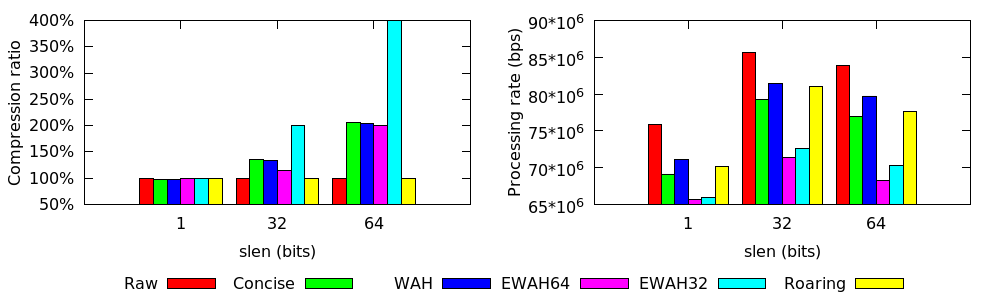
\includegraphics[width=\linewidth]{states.png}
\caption{Bitmap generation with compression algorithms}
\label{img:states}
\end{center}
\end{figure}

In the first part of the experiment, we generated the bitmaps with different algorithms and different $slen$, and then calculated the compression ratios. The result in Figure \ref{img:states} proves our deduction in Section \ref{sec:bm:compression} that when $slen < wlen$, the bitmap cannot be well compressed by any RLE-model algorithm, and in this case, the algorithm EWAH behaves a little better than the others for its smaller structure cost. When $slen$ increases to 32 and 64, i.e. $slen \geq wlen$, the RLE-model algorithms start to work and the compression ratio of $slen = 64$ is obviously better than the one of $slen = 32$. From the figure \ref{img:states} we can also see that when $slen$ is 1, 32 and 64, EWAHs are much slower than WAH, Concise and Roaring.

\begin{comment}
The result in Figure \ref{img:ratio} shows that when the length of consecutive bits is small ($\leq 5$), there is no great gap of the ratio among the RLE-model algorithms, Roaring bitmap and even uncompressed bitmap. The word lengths of WAH, Concise, EWAH(32bit), EWAH(64bit) are 32, 32, 32 and 64, so when the length grows beyond 50, which is over 32 and slightly less than 64, the ratios increase dramatically. The compression ratio of Roaring bitmap depends on the fraction of 1s bits in the bitmap, when the bitmap is not very sparse, the algorithm has to allocate much memory for its containers which in our opinion is the reason that its compression ratio is near 1 (uncompressed).
\end{comment}

In the second part, we measured the performance of the compressed bitmaps when applying the algorithms for evaluating all fundamental operators and all LTL formul\ae{}s in the previous experiments. Detailed results covering all the operators and formul\ae{}s can be found in Appendix \ref{appendixa}.

During the analyze, we picked formula F1 and F14 as the representatives, as F1 contains all the operators and connectives of LTL and F14 is the slowest formul\ae{} in the last experiment. The benchmark ran for 100 cycles; in each cycle, echo formula was executed with one group of input bitmaps from the last step and we recorded the time cost of each bitmap algorithm and each length of consecutive bits.

\begin{figure}[h]
\begin{center}
\centering
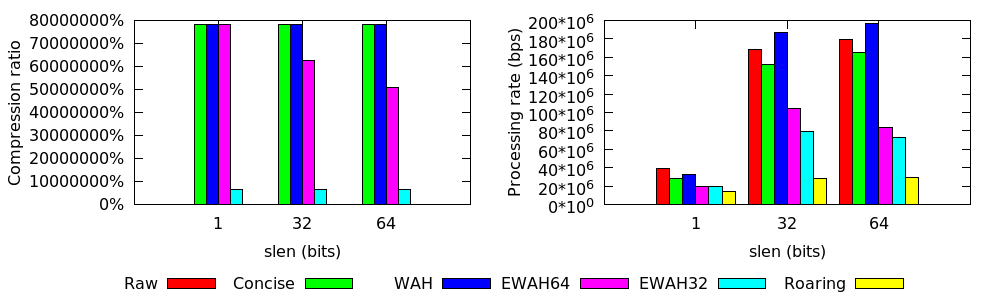
\includegraphics[width=\linewidth]{p11.png}
\caption{Formul\ae{} 1}
\label{img:f1}
\end{center}
\end{figure}

\begin{figure}[h]
\begin{center}
\centering
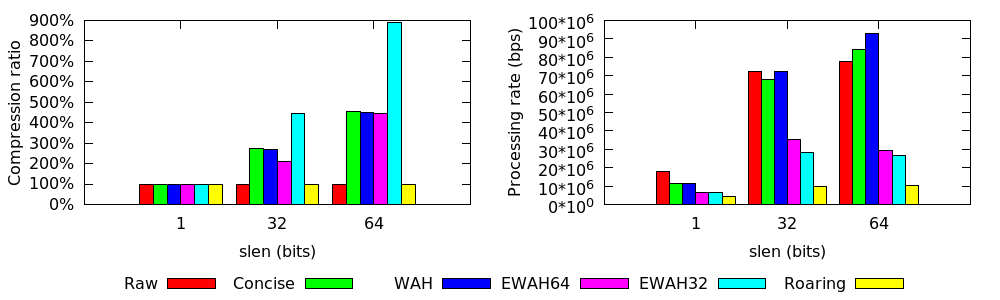
\includegraphics[width=\linewidth]{p24.png}
\caption{Formul\ae{} 14}
\label{img:f14}
\end{center}
\end{figure}

According to Figure \ref{img:f1} and \ref{img:f14}, the performance of the RLE-model algorithms, WAH, EWAH and Concise is obviously relevant to $slen$. The Figure \ref{img:f1} also suggests: the operator \G can extremely increase the consecutive length which can be well compressed by RLE-model algorithms, and several algorithms have better performance than uncompressed bitmap as $slen$ increases.

%% }}} --- Subsection

%% }}} --- Section

%% ------------------
%% Section: related work
%% ------------------
\section{Related Work}\label{sec:bm:related} %% {{{

The prospect of using physical properties of hardware to boost the performance of runtime verification has already been studied in the recent past. For example, Pellizzoni \etal\@ \cite{pellizzoni2008hardware} utilizes dedicated \emph{Commercial-OffThe-Shelf
(COTS) } hardwares and \emph{Past-time Temporal Linear Logic (PTLTL)} \citep{emerson1990temporal} to facilitate the runtime monitoring of critical embedded system.

As the number of cores (GPU or multi-core CPUs) in the commodity hardware keeps increasing, the research of exploiting the available processors or cores to parallelize the tasks and the computing  brings a challenge and also an opportunity to improve the architecture of runtime verification. For example, Ha \etal\@ \citep{ha2009concurrent} introduced a buffering design of \emph{Cache-friendly Asymmetric Buffering (CAB)} to improve the communications between application and runtime monitor by exploiting the shared cache of the mutilcore architecture; Berkovich \etal\@ \citep{DBLP:journals/fmsd/BerkovichBF15} proposed a GPU-based solution that by effectively utilizing the available cores of the GPU, the monitor designed and implemented with their method can run with the target program and evaluate the properties with LTL in parallel.

Previous work by one of the authors \citep{jocasa} introduced an algorithm for the automated verification of Linear Temporal Logic formul\ae{} on event traces, using an increasingly popular cloud computing framework called MapReduce. The algorithm can process multiple, arbitrary fragments of the trace in parallel, and compute its final result through a cycle of runs of MapReduce instances.
The proposed technique manipulates objects called \emph{tuples}, which are  of the form $\langle \psi, (n, i)\rangle$, and are interpreted as the statement ``the process is at iteration $i$, and LTL formula $\psi$ is true for the suffix of the current trace starting at its $n$-th event''. One can see that this statement corresponds exactly to the fact, in the present solution, that the $n$-th position of the bitmap generated by the evaluation of $\psi$ contains the value 1.

Apart from this similarity, however, the two techniques are radically different. Since the MapReduce approach operates on tuples one by one, while the present solution manipulates entire bitmaps, the algorithms for each LTL operator have little in common (especially that for \textbf{U}). Where the MapReduce approach gets its speed from the processing of multiple subformul\ae{} on different machines, our present solution is efficient because some operations (such as conjunction) can be computed simultaneously for many adjacent events in a single CPU cycle. Another downside of the MapReduce solution is the large number of tuples generated, and the impossibility of compressing that volume of data.


%% }}} --- Section

%% ------------------
%% Section: conclusion
%% ------------------
\section{Conclusion and future work}\label{sec:bm:conclusion} %% {{{

We proposed a solution of evaluating LTL formul\ae{} with bitmaps. The event states are mapped into bits of bitmaps which then are manipulated to implement the LTL operators. The performance benchmark of the fundamental operators and the complicated LTL formul\ae{} proved its feasibility.

To further exploit the potential of bitmap, we introduced bitmap compression algorithms in our solution and integrated them with our algorithms. In the experiments, as we expected, the compressed bitmap demonstrated its ability of compressing the sparse bitmaps and accelerating the LTL operations when there were certain amount of consecutive sequences.

This solution is designed only for the offline evaluation, and if we want to apply it on the online analysis there is still much work to do. And it is also very interesting to have the algorithms parallelized to treat huge amount of data.

%% }}} --- Section

%% :folding=explicit:wrap=soft:mode=latex:
